% Lecture Template for ME3001-001-Tristan Hill - Spring 2020
% Mechanical Engineering Analysis with MATLAB
% Ordinary Differential Equations - Lecture 1

% I am finally converting my stuff to BEAMER

% Document settings



%\documentclass{beamer}                  % for presentation ?
\documentclass[handout]{beamer}  % for handout ?
\usepackage{beamerthemesplit}
\usepackage{amsmath}
\usepackage{listings}
\usepackage{multicol}

\beamertemplateballitem

\definecolor{TTUpurple}{rgb}{0.3098, 0.1607, 0.5176} % TTU Purple (primary)
\definecolor{TTUgold}{rgb}{1.0000, 0.8666, 0.0000} % TTU Gold (primary)

\setbeamercolor{palette primary}{bg=TTUpurple,fg=TTUgold}
\setbeamercolor{palette secondary}{bg=black,fg=TTUgold}
\setbeamercolor{palette tertiary}{bg=black,fg=TTUpurple}
\setbeamercolor{palette quaternary}{bg=TTUgold,fg=black}
\setbeamercolor{structure}{fg=TTUpurple} % itemize, enumerate, etc
\setbeamercolor{section in toc}{fg=TTUpurple} % TOC sections

%\usefonttheme{professionalfonts}

\newcommand{\LNUM}{1\hspace{2mm}} % Lecture Number 

\newcommand{\secondtitle}{Review of Differential Equations}% second line of the title of this presentation , aka the topic of this lecture
\newcommand{\vspcc}{\vspace{6mm}\\ } 
\newcommand{\vspc}{\vspace{3mm}\\ } 
\newcommand{\hspc}{\hspace{5mm} } 


\title{Ordinary Differential Equations - Lecture \LNUM}
\author{ME3001 - Mechanical Engineering Analysis} % original formatting from Mike Renfro, September 21, 2004

\date{March 29, 2020}

\begin{document}

\lstset{language=MATLAB,basicstyle=\ttfamily\small,showstringspaces=false}

\frame{\titlepage \center\textbf{\secondtitle}\vspcc}

%\section*{Outlines}
%\subsection*{Part I: Review of Previous Lecture}
%\frame{
%  \nameslide{outline}
%  \frametitle{Review of Previous Lecture}
%  \tableofcontents[part=1]
%}

%\subsection*{Part II: Solution of Simultaneous Linear Algebraic Equations}
%\frame{
%  \frametitle{Solution of Simultaneous Linear Algebraic Equations}
%  \tableofcontents[part=1]
%}

%\part{Review of Previous Lecture}
%\frame{\partpage}

%\frame{
%  \frametitle{Review of Previous Lecture}

%  \begin{itemize}
%  \item<+-| alert@+> Sample problems solved with numerical methods
%    \begin{itemize}
%    \item<+-| alert@+> Natural frequencies of a vibrating bar
%    \item<+-| alert@+> Static analysis of a scaffolding
%    \item<+-| alert@+> Critical loads for buckling a column
%    \item<+-| alert@+> Realistic Design Properties of Materials
%    \end{itemize}
%  \item<+-| alert@+> Solution of nonlinear equations
%    \begin{itemize}
%    \item<+-| alert@+> Introduction
%    \item<+-| alert@+> Example: fluid mechanics
%    \item<+-| alert@+> Incremental search method
%    \end{itemize}
%  \end{itemize}
%}
%ballitem
%\part{Solution of Simultaneous Linear Algebraic Equations}
%\frame{\partpage}

\frame{

{\bf Lecture \LNUM- \secondtitle :} \vspace{3mm}\\ % ' topics' are beamer 'sections' - TWH

 \begin{itemize}
	\item Definitions\vspace{5mm}\\
	\item Classification \vspace{5mm}\\	
	\item Engineering Applications \vspace{5mm}\\
	\item Example \vspace{5mm}\\
\end{itemize}

}

\section{Definitions}

\subsection{What is a Differential Equation?}

\frame{

  \frametitle{What is a Differential Equation?}
  {\it Definition:\vspace{3mm}\\}
  A {\bf differential equation} is an equation which describes a function \vspace{3mm}\\and one or more of its \underline{\hspace{50mm}} of the \vspace{3mm}\\ \underline{\hspace{50mm}}\hspace{3mm}\underline{\hspace{50mm}}\vspace{5mm} \\ with respect to the \underline{\hspace{60mm}}.

}


\subsection{Standard Form of an ODE}

\frame{

  \frametitle{Standard Form of an ODE}

  Ordinary Differential Equations are written in the following form.\vspace{3mm}\\

\scalebox{1.2}{$a_n\frac{dy^{(n)}}{d^{(n)}x}+a_{n-1}\frac{dy^{(n-1)}}{d^{(n-1)}x}+...+a_{2}\frac{dy^{2}}{d^{2}x}+a_{1}\frac{dy}{dx}+a_0y=f(x)$}	\vspace{0mm}\\		

The apostrophe is commonly used for the derivative. \vspace{2mm}\\

\scalebox{1.2}{$a_ny^{(n)}+a_{n-1}y^{(n-1)}+...+a_2y'' +a_1y'+a_0y=f(x)$} \vspace{3mm}\\

If time is the independent variable the equation changes slightly. \vspace{2mm}\\



}


\section{Classification}

\subsection{Ordinary or Partial}

\frame{
  
  \frametitle{Is the differential equation ordinary or partial?}

An {\bf ordinary} differential equation has \underline{\hspace{20mm}} independent \vspc variable and \underline{\hspace{20mm}} dependent variable. \vspace{10mm}\\

A {\bf partial} differential equation has \underline{\hspace{50mm}} \vspc independent variable  \underline{\hspace{20mm}}  dependent variable. \vspace{10mm}\\

}

\subsection{Order}

\frame{
  
  \frametitle{What is the order of the equation?}
  
The {\bf order} of a differential equation is the \vspace{3mm}\\ \underline{\hspace{50mm}}\hspace{3mm}\underline{\hspace{50mm}} \vspace{5mm}\\ present in the equation. \vspace{3mm}\\

}

\subsection{Degree}

\frame{
  
  \frametitle{What is the degree of the equation?}

The {\bf degree} of a differential equation is the \underline{\hspace{30mm}}\hspace{3mm} \vspace{5mm}\\ of its highest derivative, after the equation has been made rational \vspace{5mm}\\ and integral in all of its derivatives. \vspace{3mm}\\


}


\subsection{Linear or Non-Linear}

\frame{
  
\frametitle{Is the differential equation linear or non-linear?}

An ordinary differential equation is \underline{\hspace{30mm}} if the following statements are true. \vspace{5mm}\\

\begin{enumerate}
\item {\it The dependent variable and its derivatives are of the first degree.} \vspace{3mm}\\

\item {\it The coefficients are constants or dependent on the independent variable.}\vspace{3mm}\\
\end{enumerate}

If either rule is broken, the equation is \underline{\hspace{10mm}}-\underline{\hspace{30mm}}.

}


\section{Engineering Applications}
\frame{
  
\frametitle{Engineering Applications}

Differential equations are used to describe physical systems in many areas of engineering. An equation that represents a physical (or theoretical) system is known as a \underline{\hspace{50mm}}\hspace{3mm}\underline{\hspace{50mm}}.\vspace{3mm}\\
\begin{itemize}

	\item Solid Mechanics \vspace{3mm}\\
	\item Kinematics and Dynamics \vspace{3mm}\\
	\item Heat Transfer and Thermodynamics \vspace{3mm}\\
	\item Fluid Mechanics
			
\end{itemize}

}


\section{Example}

\subsection{Example - Mathematical Model}
\frame{

\frametitle{Example - Mathematical Model}

\begin {multicols}{2}

Newton's Second Law \vspace{2mm}\\

$\Sigma {\bf F}=m {\bf a}$ \vspace{2mm}\\

leads  to an {\it equation of motion}.  \vspace{2mm}\\

$\dot{y}+\frac{c}{m}y=f(t)$

 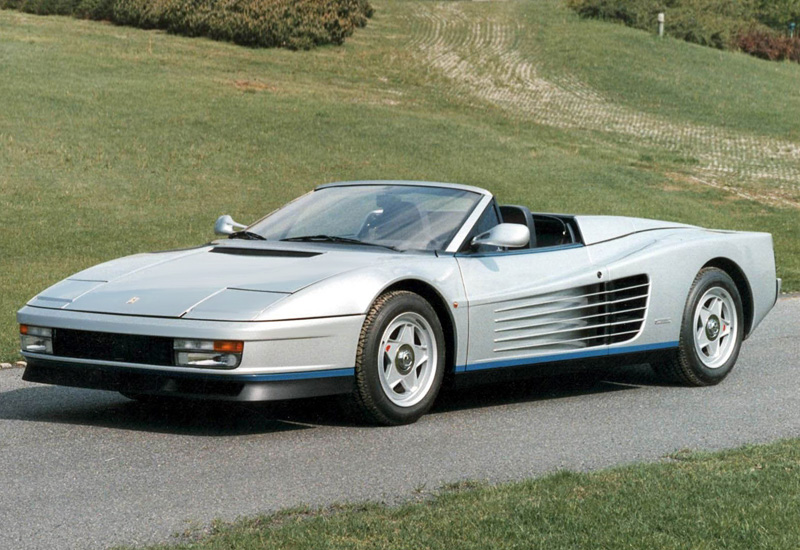
\includegraphics[scale=0.15]{ferrari.jpg}\\
 
 \end{multicols} 
  

}

\subsection{Example - Solution}
\frame{

\frametitle{Example -  Solution}



The {\bf solution} to a differential equation describes the \vspace{2mm}\\ \underline{\hspace{40mm}}\hspace{2mm}\underline{\hspace{40mm}} as a function \vspace{2mm}\\of the \underline{\hspace{40mm}}\hspace{2mm}\underline{\hspace{40mm}}.  \vspace{5mm}\\


	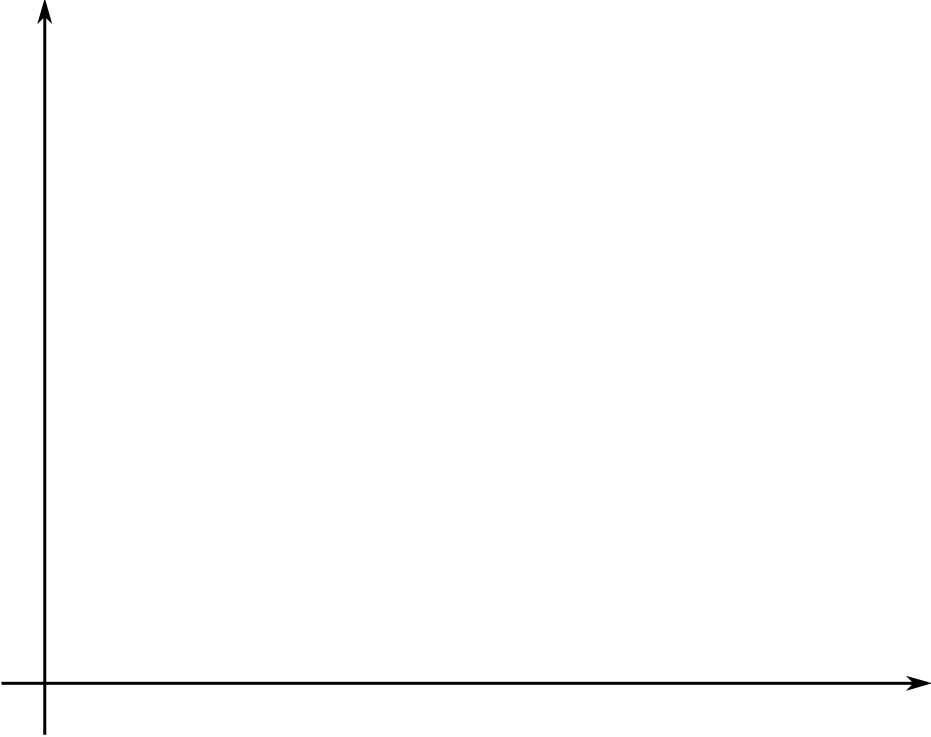
\includegraphics[scale=0.10]{lecture1_fig2.png} \hspace{10mm} 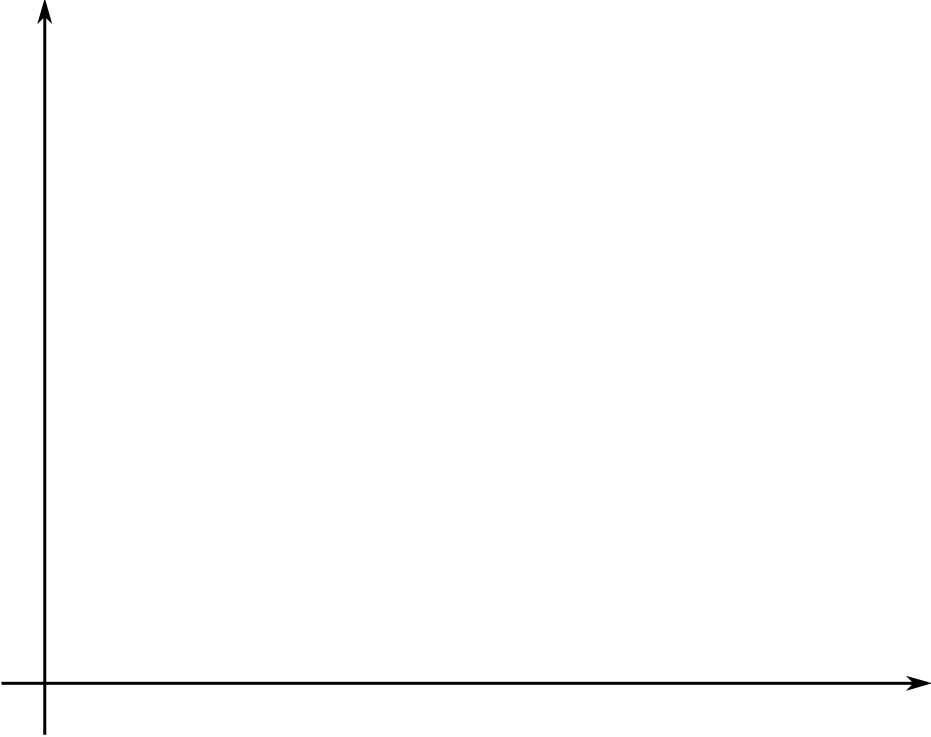
\includegraphics[scale=0.10]{lecture1_fig2.png}\vspace{2mm}\\
	
	%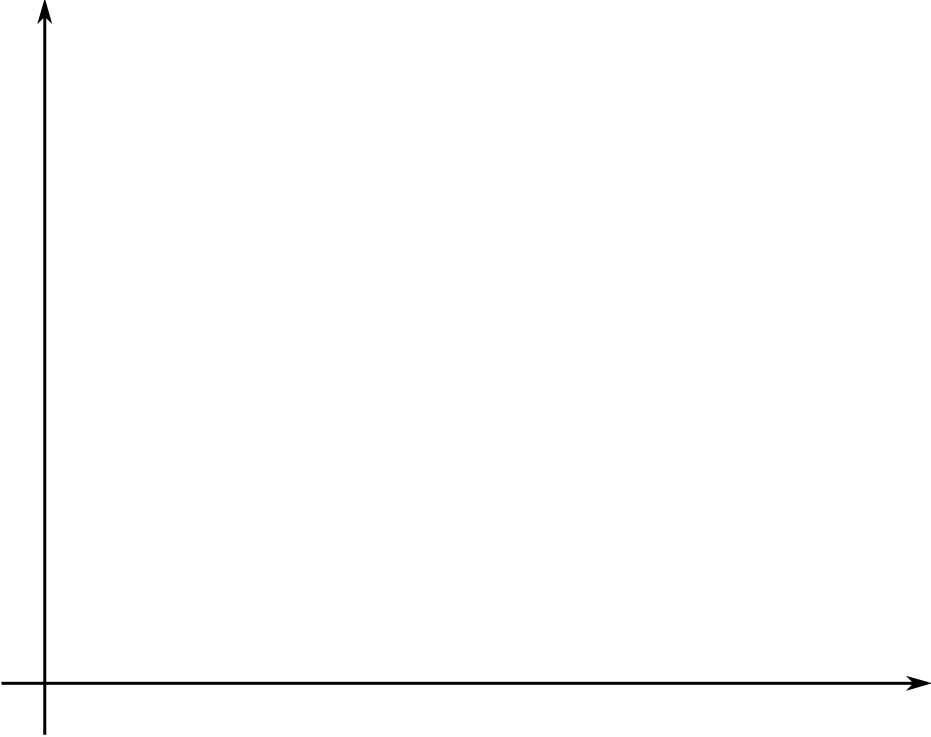
\includegraphics[scale=0.1]{lecture1_fig2.png}\\	
	
There are many different methods for finding the solution.
  

}

\end{document}









